% \documentclass[aspectratio=169,notes]{beamer}
\documentclass[aspectratio=169]{beamer}
\usetheme[faculty=phil]{fibeamer}
\usepackage{polyglossia}
\setmainlanguage{english} %% main locale instead of `english`, you
%% can typeset the presentation in either Czech or Slovak,
%% respectively.
\setotherlanguages{russian} %% The additional keys allow
%%
%%   \begin{otherlanguage}{czech}   ... \end{otherlanguage}
%%   \begin{otherlanguage}{slovak}  ... \end{otherlanguage}
%%
%% These macros specify information about the presentation
\title[AGLA2]{Analytical Geometry and Linear Algebra II, Lab 10} %% that will be typeset on the
\subtitle{Symmetric matrices \\ Positive definite matrices and minima \\ \ 
         } %% title page.
\author{Oleg Bulichev}
%% These additional packages are used within the document:
\usepackage{ragged2e}  % `\justifying` text
\usepackage{booktabs}  % Tables
\usepackage{tabularx}
\usepackage{tikz}      % Diagrams
\usetikzlibrary{calc, shapes, backgrounds}
\usepackage{amsmath, amssymb}
\usepackage{url}       % `\url`s
\usepackage{listings}  % Code listings
% \usepackage{subfigure}
\usepackage{floatrow}
\usepackage{subcaption}
\usepackage{mathtools}
\usepackage{todonotes}
\usepackage{fontspec}
\usepackage{multicol}
\usepackage{pdfpages}
\usepackage{wrapfig}
\usepackage{animate}
\usepackage{booktabs}
\usepackage{multirow}

\graphicspath{{resources/}}
\frenchspacing

\setbeamertemplate{caption}[numbered]
\usetikzlibrary{graphs}

% \usepackage[backend=biber,style=ieee,autocite=footnote]{biblatex}
% \addbibresource{biblio.bib}
% \DefineBibliographyStrings{english}{%
%   bibliography = {References},}

\newcommand{\oleg}[2][] {\todo[color=red, #1] {OLEG:\\ #2}}
\newcommand{\fbckg}[1]{\usebackgroundtemplate{\includegraphics[width=\paperwidth]{#1}}}%frame background

\usepackage[framemethod=TikZ]{mdframed}
\newcommand{\dbox}[1]{
\begin{mdframed}[roundcorner=3pt, backgroundcolor=yellow, linewidth=0]
\vspace{1mm}
{#1}
\vspace{1mm}
\end{mdframed}
}

\begin{document}
\setlength{\abovedisplayskip}{0pt}
\setlength{\belowdisplayskip}{0pt}
\setlength{\abovedisplayshortskip}{0pt}
\setlength{\belowdisplayshortskip}{0pt}

\fbckg{fibeamer/figs/title_page.png}
\frame[c]{\setcounter{framenumber}{0}
    \usebeamerfont{title}%
    \usebeamercolor[fg]{title}%
    \begin{minipage}[b][6.5\baselineskip][b]{\textwidth}%
        \textcolor{black}{\raggedright\inserttitle}
    \end{minipage}
    % \vskip-1.5\baselineskip

    \usebeamerfont{subtitle}%
    \usebeamercolor[fg]{framesubtitle}%
    \begin{minipage}[b][3\baselineskip][b]{\textwidth}
        \raggedright%
        \insertsubtitle%
    \end{minipage}
    \vskip.25\baselineskip
}
%   \frame[c]{\maketitle}

\fbckg{fibeamer/figs/common.png}

\begin{frame}[c]{How I spent last weekend}
    \framesubtitle{}
    \begin{figure}[H]
        \begin{subfigure}{0.29\textwidth}
            \centering
\includegraphics[height=5.5cm,width=1\textwidth,keepaspectratio]{death_door.jpg}
            % \caption*{\Large Watched both seasons in 1 day \\ (24 series) of "Mushoku Tensei"}
        \end{subfigure}
        \hfill
        \begin{subfigure}{0.29\textwidth}
            \centering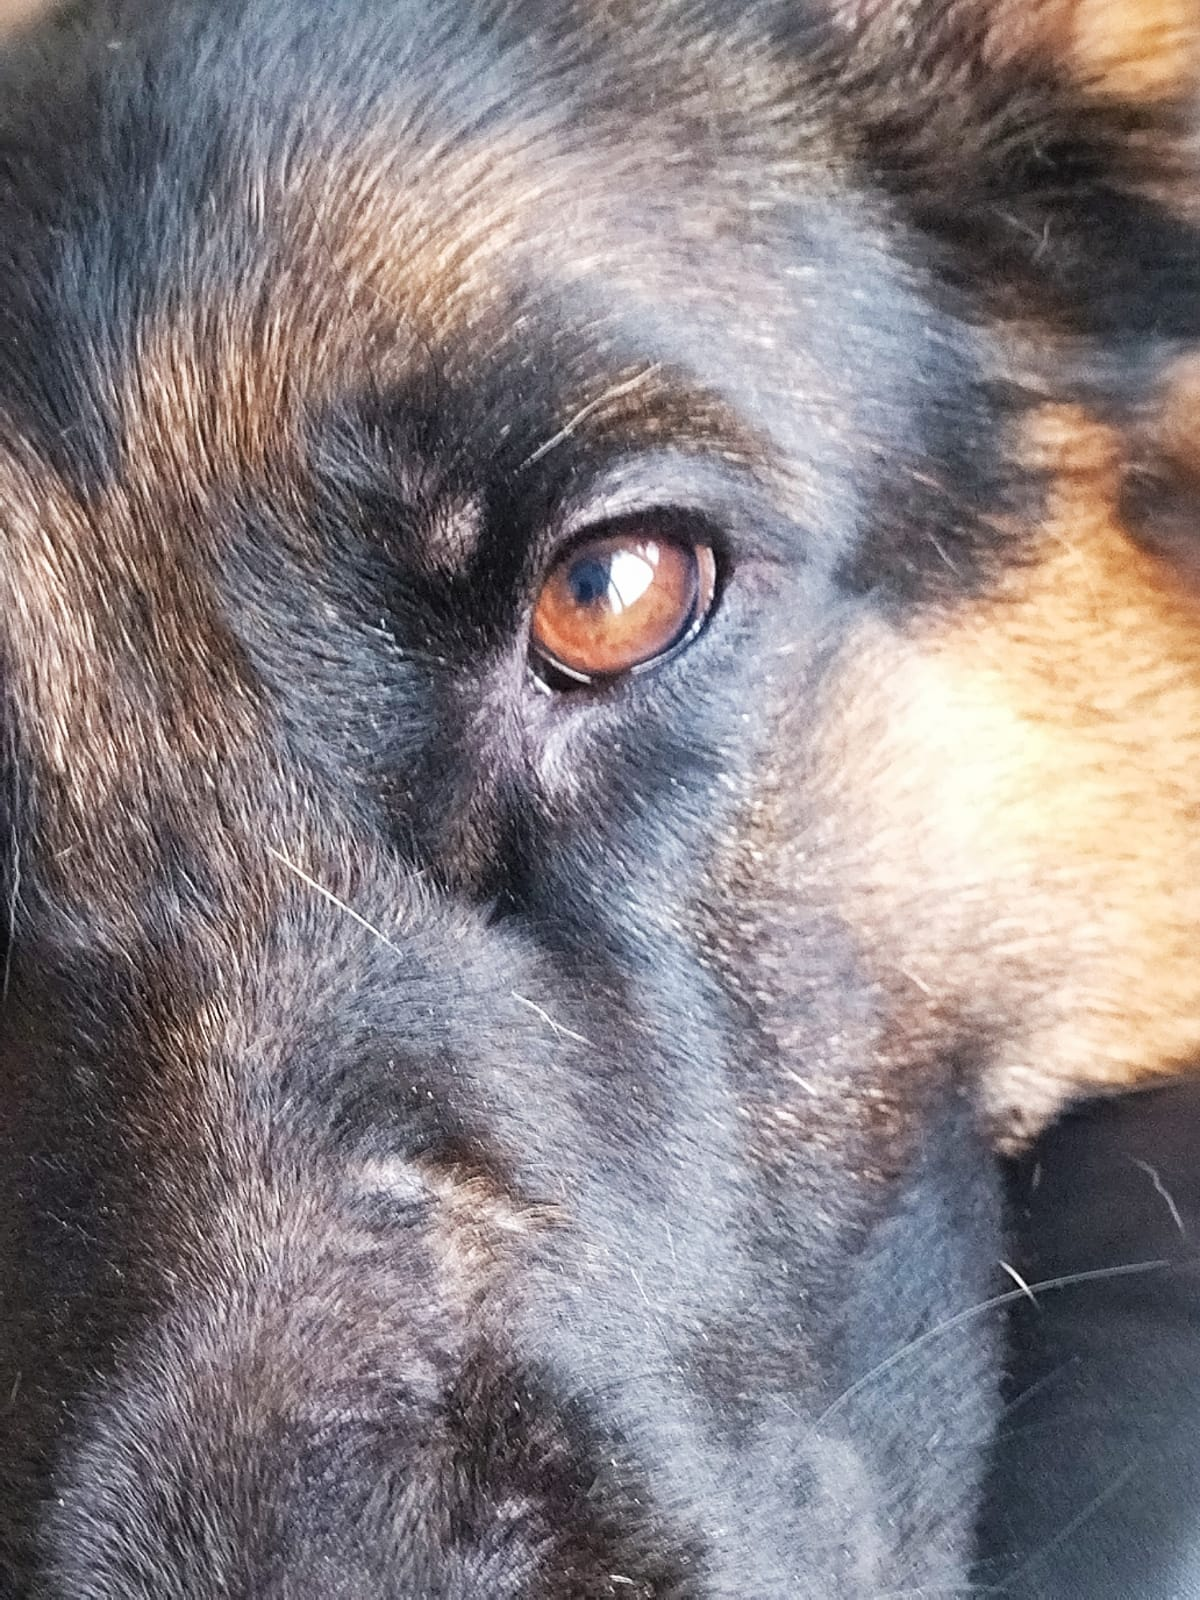
\includegraphics[height=5.5cm,width=1\textwidth,keepaspectratio]{yarik.jpg}
            % \caption*{\Large RAGE and VEGs clubs cooking collaboration event}
        \end{subfigure}        
        \hfill
        \begin{subfigure}{0.29\textwidth}
            \centering
\includegraphics[height=5.5cm,width=1\textwidth,keepaspectratio]{tunic_game.jpeg}
            % \caption*{\Large RAGE and VEGs clubs cooking collaboration event}
        \end{subfigure}
    \end{figure}
\end{frame}

\begin{frame}[t]{Symmetric Matrices (1)}
\framesubtitle{}
    \begin{figure}[H]
        \centering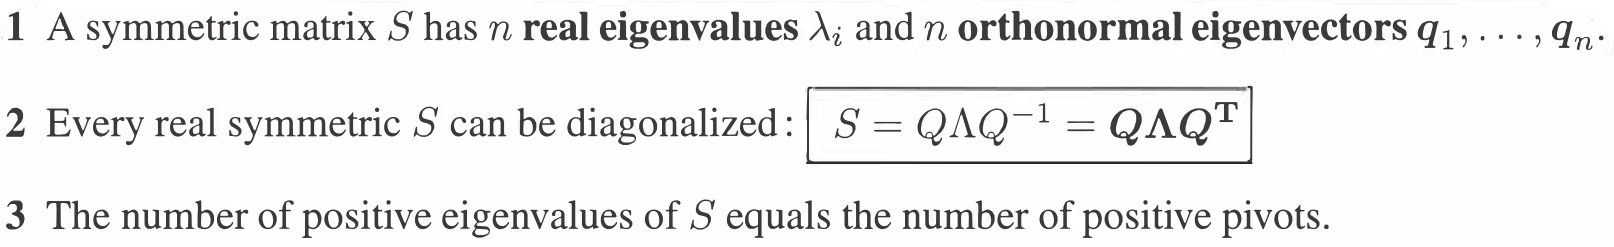
\includegraphics[height=6cm,width=1\textwidth,keepaspectratio]{symmetric.png}
        % \caption{caption_name}
        \label{fig:symmetric.png}
    \end{figure}
\end{frame}

\begin{frame}[t]{Symmetric Matrices (2)}
    \framesubtitle{}
        \begin{figure}[H]
            \centering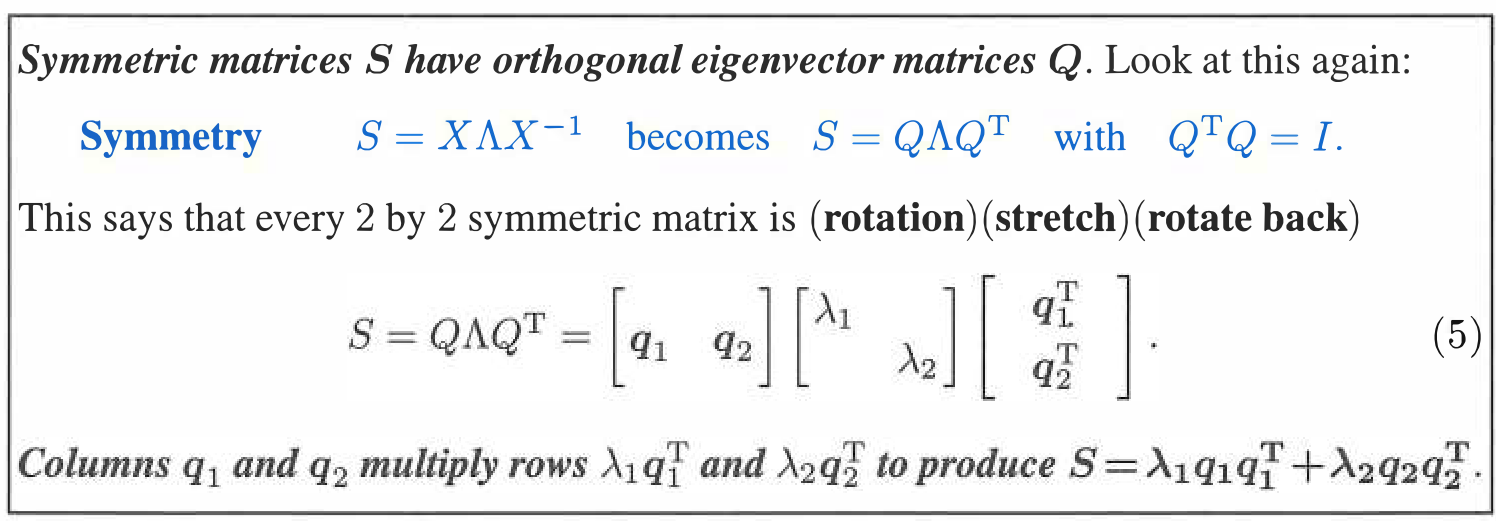
\includegraphics[height=6cm,width=1\textwidth,keepaspectratio]{symmetric_2.png}
            % \caption{caption_name}
            \label{fig:symmetric_2.png}
        \end{figure}
    \end{frame}

\begin{frame}[t]{Task 1}
    \framesubtitle{}
    \vspace{-0.5cm}
    \begin{figure}[H]
        \centering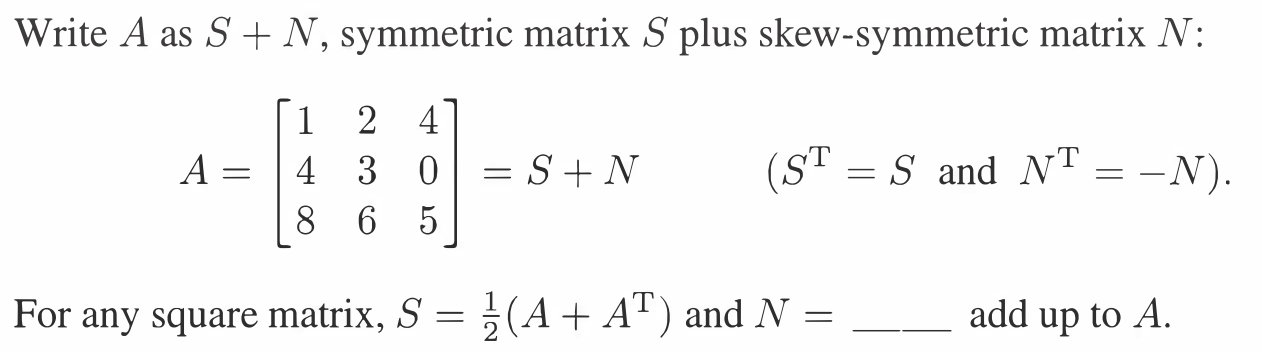
\includegraphics[height=3cm,width=1\textwidth,keepaspectratio]{1.png}
        % \caption{caption_name}
        \label{fig:1.png}
    \end{figure}
    \uncover<2->{
        \alert{\Large Answer}
        \begin{figure}[H]
            \centering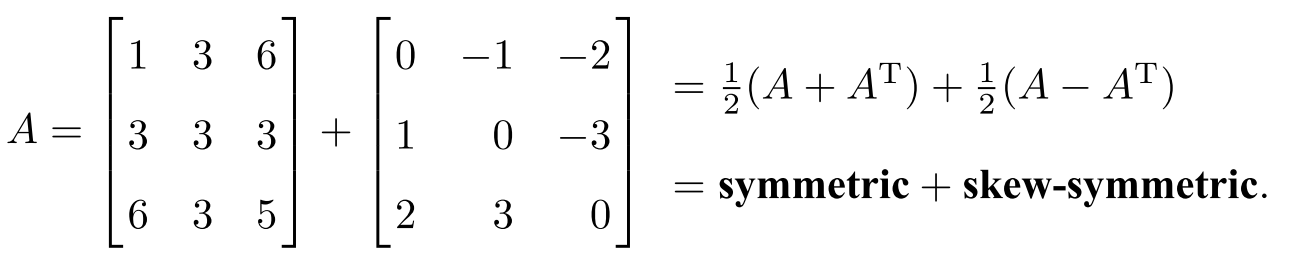
\includegraphics[height=2cm,width=1\textwidth,keepaspectratio]{1ans.png}
            % \caption{caption_name}
            \label{fig:1ans.png}
        \end{figure}
    }
\end{frame}

\begin{frame}[t]{Task 2}
    \framesubtitle{}
    \vspace{-0.5cm}
    \begin{figure}[H]
        \centering
\includegraphics[height=3cm,width=1\textwidth,keepaspectratio]{2.png}
        % \caption{caption_name}
        \label{fig:2.png}
    \end{figure}
    \uncover<2->{
        \alert{\Large Answer}
        \begin{figure}[H]
            \centering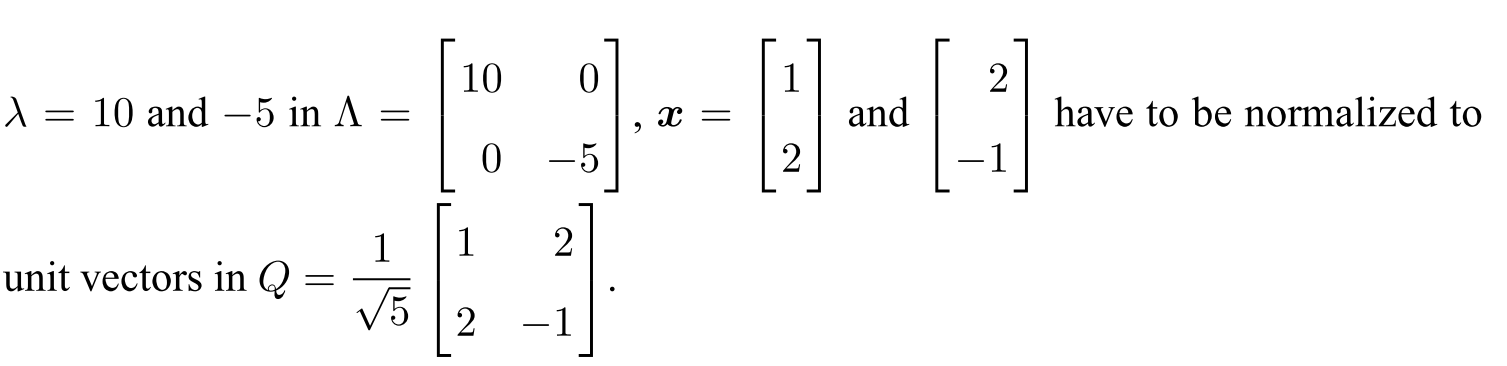
\includegraphics[height=3cm,width=1\textwidth,keepaspectratio]{2ans.png}
            % \caption{caption_name}
            \label{fig:2ans.png}
        \end{figure}
    }
\end{frame}

\begin{frame}[t]{Task 3}
    \framesubtitle{}
    \vspace{-0.5cm}
    \begin{figure}[H]
        \centering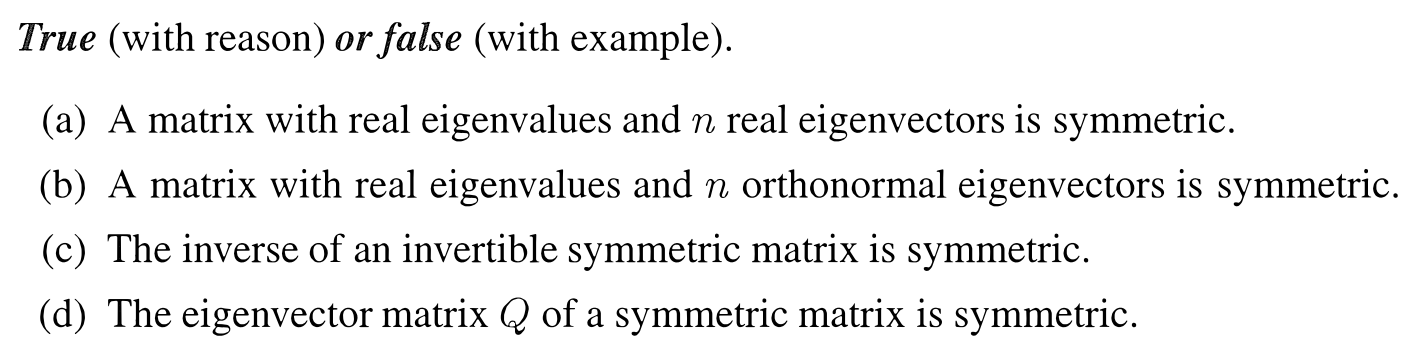
\includegraphics[height=3cm,width=1\textwidth,keepaspectratio]{3.png}
        % \caption{caption_name}
        \label{fig:3.png}
    \end{figure}
    \uncover<2->{
        \alert{\Large Answer}
        \begin{figure}[H]
            \centering
\includegraphics[height=3cm,width=1\textwidth,keepaspectratio]{3ans.png}
            % \caption{caption_name}
            \label{fig:3ans.png}
        \end{figure}
    }
\end{frame}

\begin{frame}[t]{Positive Definite Matrices}
\framesubtitle{}
    
\end{frame}


\begin{frame}[t]{Positive Definite Matrices}
    \framesubtitle{Applications from ML}
    \Large
    \begin{itemize}
        \item \href{https://en.wikipedia.org/wiki/Cholesky_decomposition}{Cholesky decomposition} -- $A=LL^H$ (A special case of $A=LU$)
        \item Least squares computation reduction
        \item \href{https://en.wikipedia.org/wiki/Support-vector_machine}{Support Vector Machine (SVM)}, \textit{kernel} -- \href{https://en.wikipedia.org/wiki/Positive-definite_kernel}{Positive-definite kernel}
        \item \href{https://analyticsindiamag.com/what-is-representer-theorem-in-machine-learning/}{Representer Theorem} 
    \end{itemize}
\end{frame}

\begin{frame}[t]{Positive Definite Matrices}
\framesubtitle{Five tests}
    \begin{figure}[H]
        \centering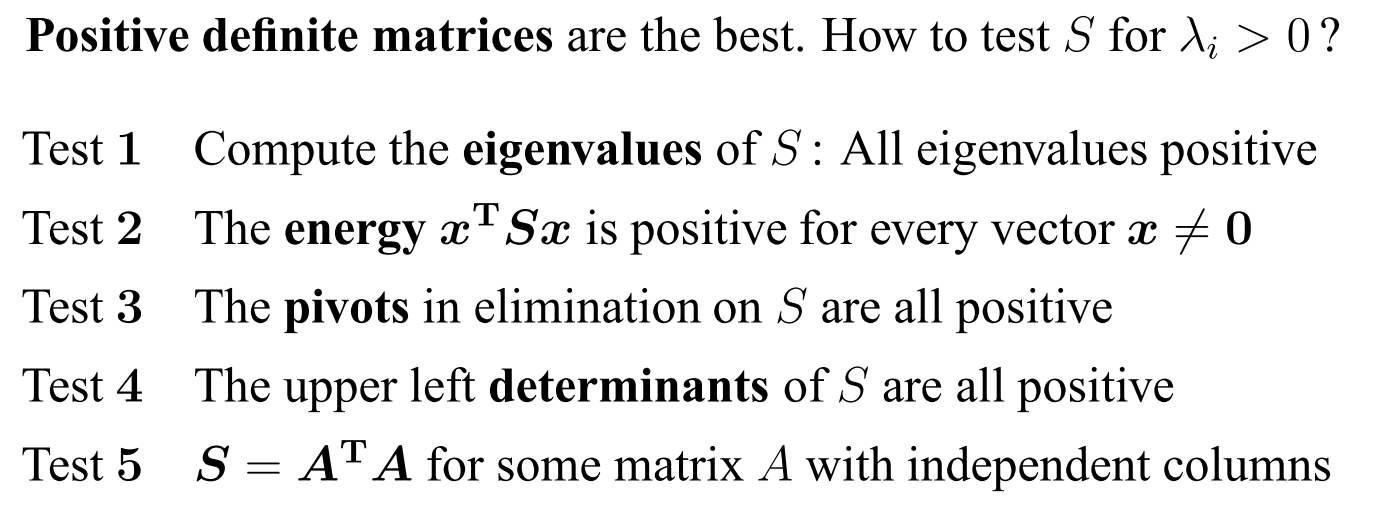
\includegraphics[height=6cm,width=1\textwidth,keepaspectratio]{positive_definite_tests.png}
        % \caption{caption_name}
        \label{fig:positive_definite_tests.png}
    \end{figure}
\end{frame}

\begin{frame}[t]{Positive Definite Matrices}
\framesubtitle{Applications from Robotics}
    \begin{itemize}
        \item \href{http://www.diag.uniroma1.it/~deluca/rob2_en/03_LagrangianDynamics_1.pdf}{Matrix form of Lagrange}
    \end{itemize}
\end{frame}


\begin{frame}[t]{Positive Definite Matrices}
    \framesubtitle{Important Application: Test for a Minimum}
    \vspace{-0.5cm}
        \begin{figure}[H]
            \centering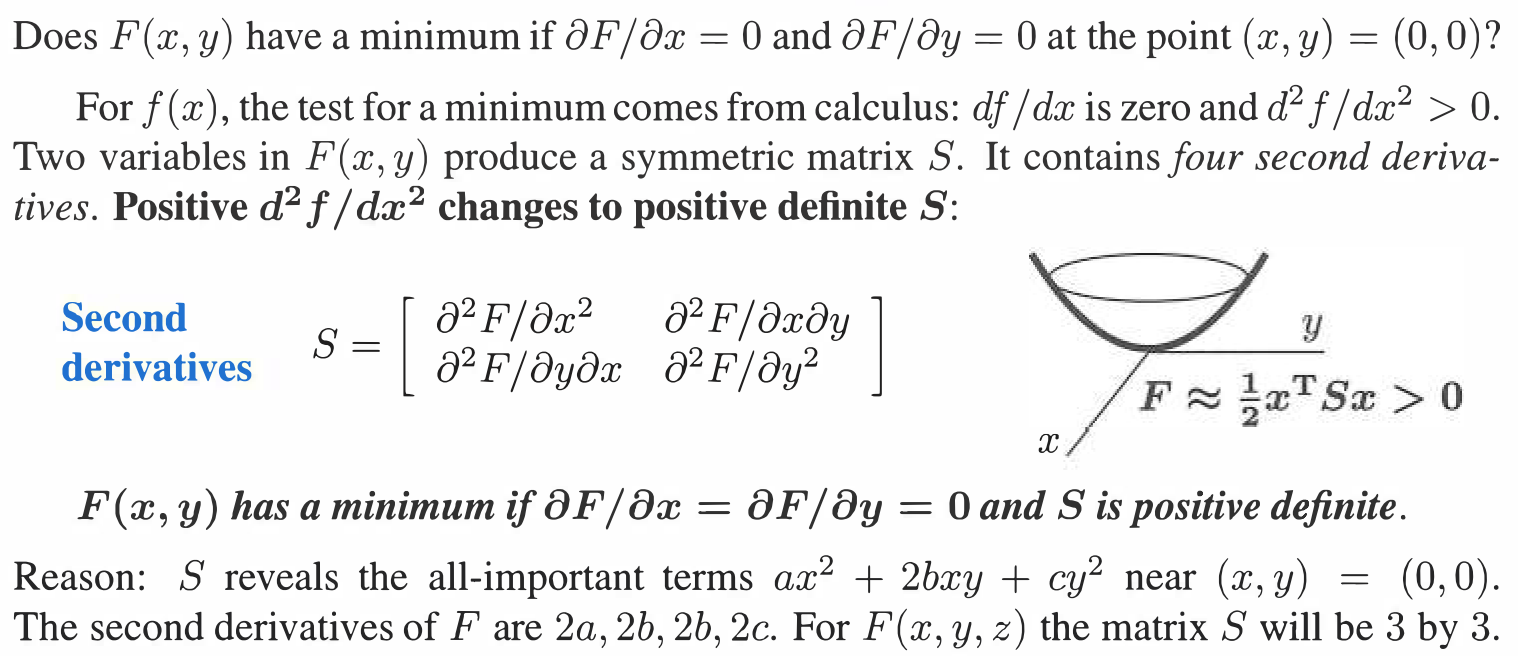
\includegraphics[height=6cm,width=1\textwidth,keepaspectratio]{test_for_minimum.png}
            % \caption{caption_name}
            \label{fig:test_for_minimum.png}
        \end{figure}
    \end{frame}

\begin{frame}[t]{Reference material}
    \framesubtitle{}
    \Large
    \begin{itemize}
        \item \href{https://www.youtube.com/watch?v=vF7eyJ2g3kU&list=PL49CF3715CB9EF31D&index=28}{Lecture 28, Positive Definite Matrices and Minima}
        \item \textit{"Introduction to Linear Algebra", pdf pages 349--374 }\\  6.4 -- Symmetric, 6.5 -- Positive Definite matrices
        \item \textit{"Linear Algebra and Applications", pdf pages 355--376 }\\ Positive Definite Matrices 6.1, 6.2
    \end{itemize}
\end{frame}

\fbckg{fibeamer/figs/last_page.png}
\frame[plain]{}

\end{document}